\documentclass[12pt,a4paper]{article}
\usepackage[utf8]{inputenc}
\usepackage{graphicx}
\usepackage{hyperref}
\usepackage{xcolor}
\usepackage{geometry}
\usepackage{setspace}
\usepackage{caption}

\geometry{margin=1in}
\setstretch{1.3}

\begin{document}

\begin{titlepage}
\centering
{\LARGE \textbf{Report: Big Data Stock Price Analysis}}\\[2cm]
{\large Analysis of VNStock Data Using Hadoop \& Spark}\\[1cm]
{\large \textbf{Data Source: VNStock (2015–2025)}}\\[2cm]
\textbf{Author:} Trinh Tuan Ngoc Bao\\[0.5cm]
\textbf{Institution:} University of Engineering and Technology – Big Data\\[0.5cm]
\textbf{Date:} \today
\end{titlepage}

\tableofcontents
\newpage

\begin{abstract}
This report presents the development of a distributed Big Data analytics system for analyzing Vietnamese stock market data from VNStock.
The project demonstrates an end-to-end data pipeline including data collection, storage, preprocessing, and distributed analysis on a Docker-based Hadoop–Spark cluster.
The system efficiently handles thousands of stock records and performs analytical tasks such as price trend tracking and growth rate comparison across major Vietnamese bank stocks.
\end{abstract}

%-----------------------------------
\section{Introduction}

The Vietnamese stock market has expanded rapidly in both transaction volume and market capitalization.  
Consequently, traditional data processing tools struggle to handle the growing scale and velocity of market data.  

This project builds a simulated Big Data environment for analyzing stock prices using VNStock as the primary data source.  
It integrates \textbf{Hadoop Distributed File System (HDFS)} for scalable storage and \textbf{Apache Spark} for distributed computation.  
The approach demonstrates the benefits of Big Data technologies in managing and analyzing financial time-series data efficiently.

%-----------------------------------
\section{Theoretical Background}

\subsection{Big Data Systems}
Big Data refers to datasets with massive volume, variety, and velocity, which require distributed systems for efficient storage and analysis.  
Frameworks such as Hadoop and Spark enable horizontal scalability and high processing speed.

\subsection{Hadoop and HDFS}
Hadoop provides distributed data storage through HDFS, allowing large files to be partitioned across multiple DataNodes.  
A central NameNode manages metadata, ensuring fault tolerance and high availability.

\subsection{Apache Spark}
Apache Spark is an in-memory data processing engine designed for large-scale distributed computation.  
It performs transformations and aggregations much faster than traditional MapReduce, making it ideal for iterative analytics tasks such as stock trend analysis.

\subsection{Stock Data Characteristics}
Stock market data are a form of time-series data — values recorded sequentially over time.  
They are highly dynamic and influenced by numerous market factors, requiring efficient systems for continuous collection and processing.

%-----------------------------------
\section{System Design and Implementation}

\subsection{System Architecture}
The system was deployed using Docker Compose and consists of:

\begin{itemize}
    \item \textbf{HDFS Cluster:} 1 NameNode and 4 DataNodes to store distributed data.
    \item \textbf{Spark Cluster:} 1 Spark Master and 4 Spark Workers for distributed computation.
    \item \textbf{Jupyter Notebook:} interactive interface for accessing the Spark cluster.
\end{itemize}

\begin{figure}[h!]
    \centering
    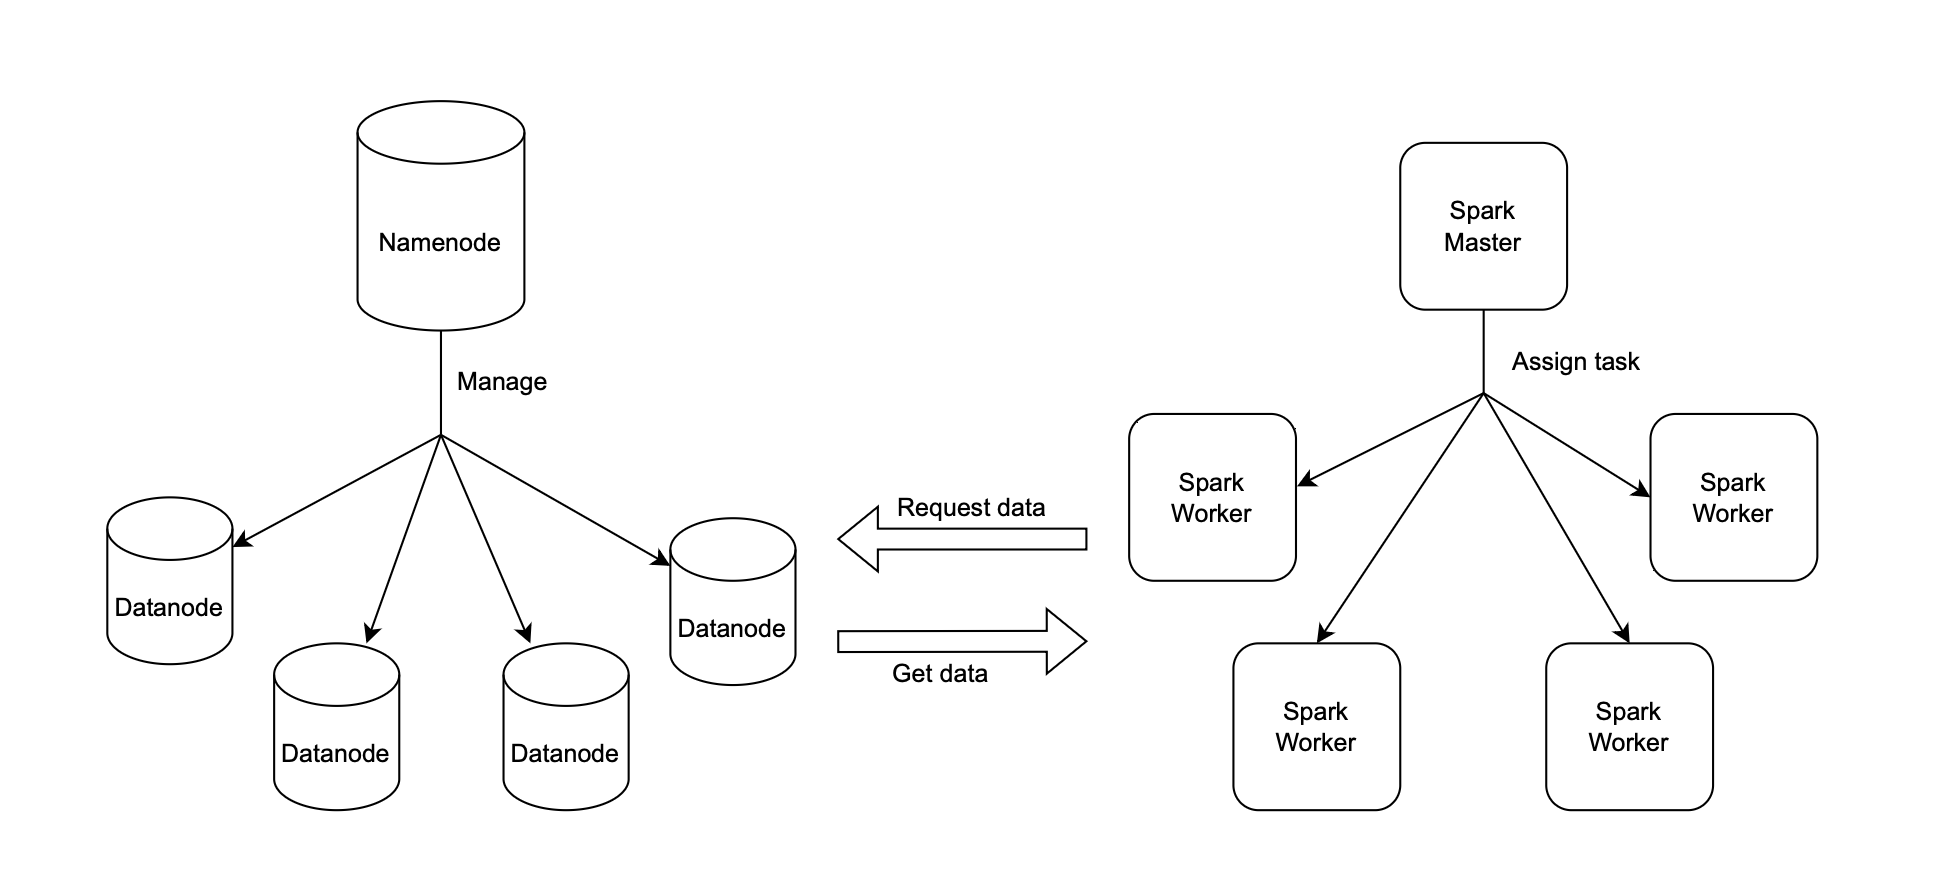
\includegraphics[width=0.9\textwidth]{architecture.png}
    \caption{System architecture integrating Hadoop and Spark clusters.}
\end{figure}

\subsection{Cluster Setup}
Each node is deployed as a Docker container using the following images:

\begin{itemize}
    \item \texttt{bde2020/hadoop-namenode:2.0.0-hadoop3.2.1-java8}
    \item \texttt{bde2020/hadoop-datanode:2.0.0-hadoop3.2.1-java8}
    \item \texttt{spark:3.5.0} (for both Master and Workers)
    \item \texttt{jupyter/pyspark-notebook:latest}
\end{itemize}

This setup allows distributed processing and scalability across multiple nodes in a controlled environment.

%-----------------------------------
\section{Data Collection}

The dataset consists of daily stock prices collected from VNStock for 10 major banks:

\begin{center}
VCB, BID, CTG, TCB, MBB, ACB, VPB, HDB, STB, SHB
\end{center}

Data includes fields such as \textit{time, open, high, low, close, volume}, spanning the period from 2015 to 2025.  
Each stock’s data was saved as CSV and uploaded to HDFS for distributed analysis.

%-----------------------------------
\section{Data Preprocessing}

Before analysis, the data underwent several cleaning and transformation steps:

\begin{itemize}
    \item Convert date strings into \texttt{datetime} format.
    \item Remove missing or invalid records.
    \item Normalize stock symbols and price columns.
    \item Filter the dataset to focus on the banking sector for consistent comparison.
\end{itemize}

These preprocessing steps ensure data consistency and reliability before Spark-based processing.

%-----------------------------------
\section{Data Analysis}

\subsection{Price Trend Analysis}
The closing price trend for each bank was analyzed to visualize performance over time.  
The figure below illustrates how selected banking stocks evolved between 2015 and 2025.

\begin{figure}[h!]
    \centering
    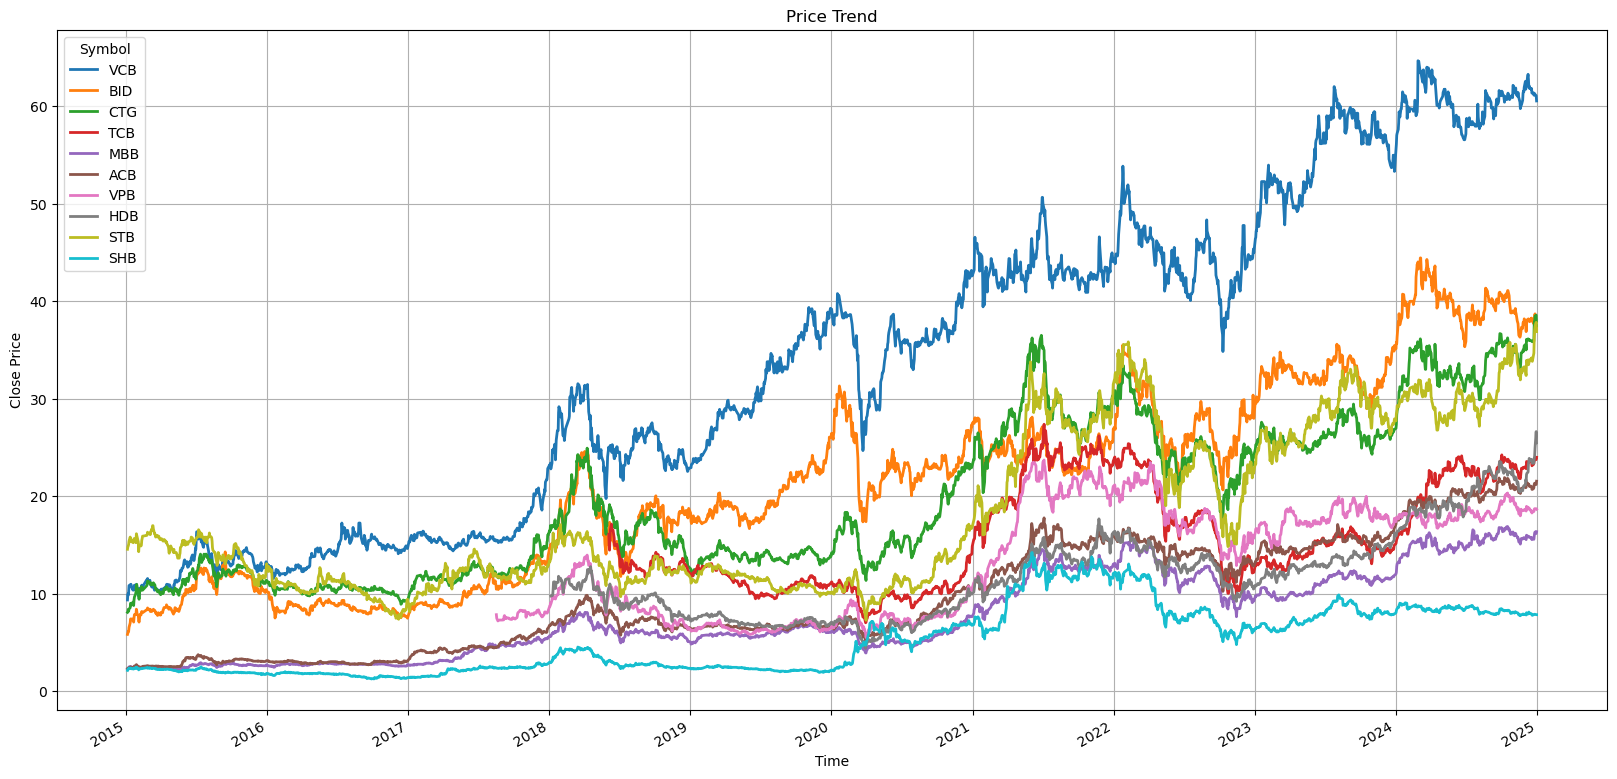
\includegraphics[width=0.9\textwidth]{price_trend.png}
    \caption{Price trends of major Vietnamese bank stocks (2015–2025).}
    \label{fig:trend}
\end{figure}

\textbf{Discussion:}  
The analysis reveals that most major bank stocks—particularly VCB, BID  a steady increase in price over the long term, despite temporary fluctuations during market corrections.  
Stocks like VCB and MBB exhibited strong resilience and long-term stability, reflecting solid fundamentals and investor confidence.

\subsection{Price Growth Rate Analysis}
The two-month price growth rate was computed to evaluate short-term and medium-term volatility among different bank stocks.

\begin{figure}[h!]
    \centering
    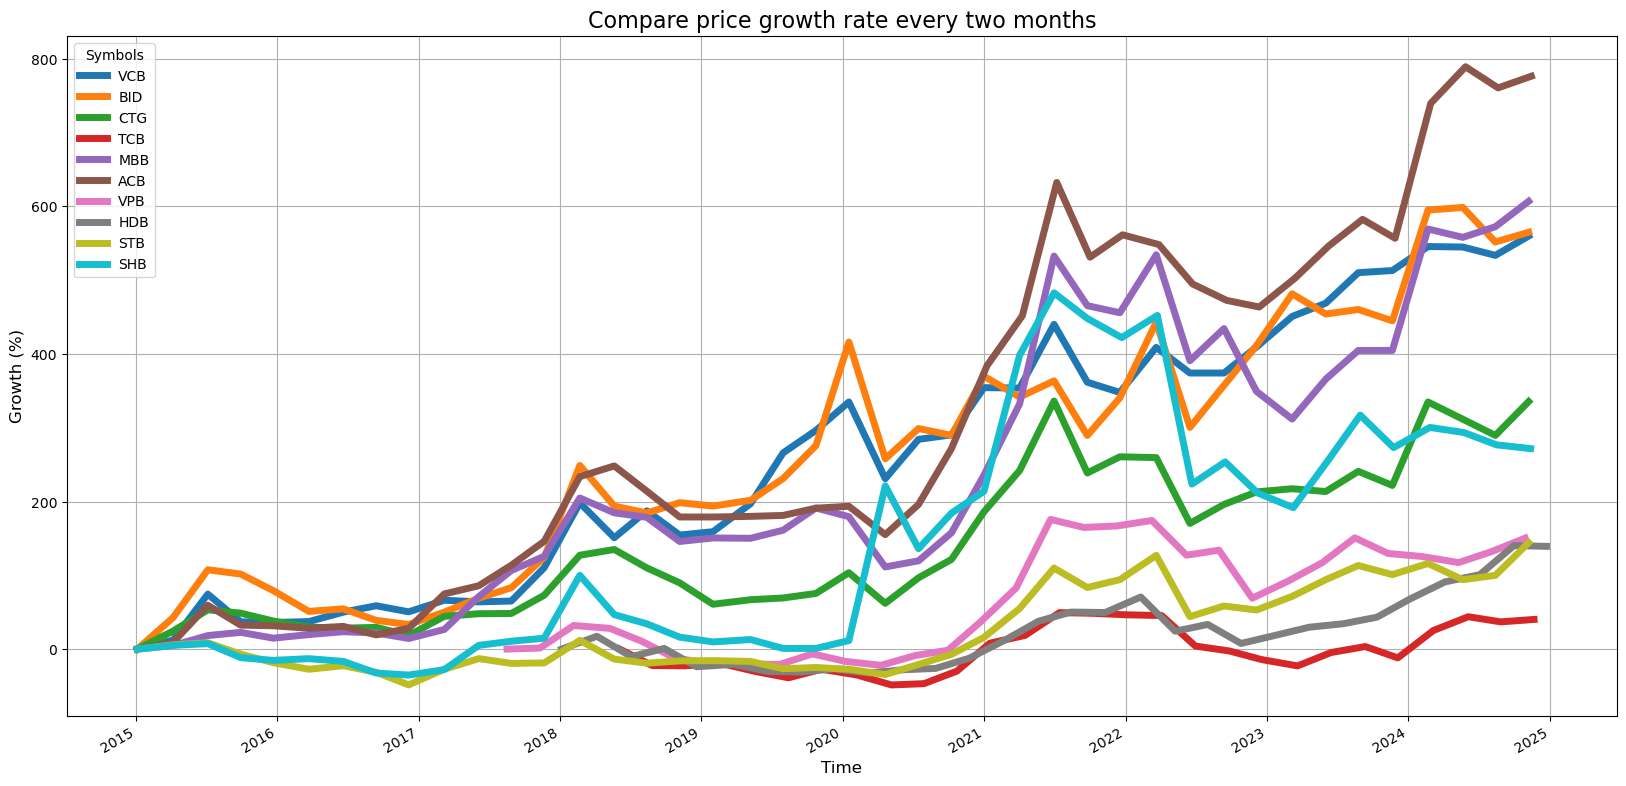
\includegraphics[width=0.9\textwidth]{price_growth_rate.png}
    \caption{Two-month price growth rate comparison among bank stocks.}
    \label{fig:growth}
\end{figure}

\textbf{Discussion:}  
The growth rate analysis highlights varying levels of volatility.  
Stocks like ACB and MBB demonstrate high fluctuations, implying higher risk but potential for speculative gains.  
Conversely, ACB and BID maintain smoother growth trajectories, indicating stable long-term investments.  
These insights can guide investment decisions based on risk tolerance and growth consistency.

%-----------------------------------
\section{Conclusion}

This report presents the design and implementation of a Big Data analytics system for analyzing VNStock data using Hadoop and Spark.  
The system demonstrates efficient data collection, preprocessing, and distributed computation capabilities.  

Through analyses of price trends and growth rates, the study identifies differences in market behavior among leading Vietnamese banks.  
The results confirm that distributed Big Data technologies are effective tools for large-scale financial analytics and provide valuable insights for investors and researchers.

\vspace{1cm}
GitHub: \url{https://github.com/ngocbao220/Bigdata-ASM1-StockPrice}
\end{document}
